\begin{figure}[H]
    \centering



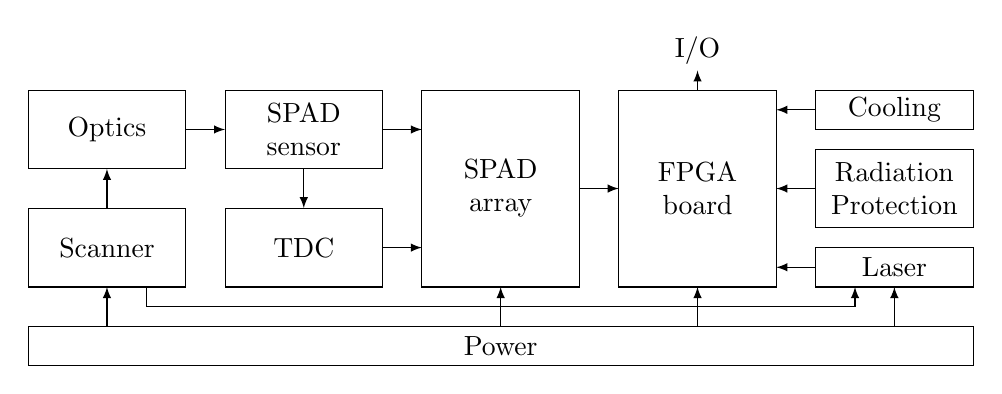
\begin{tikzpicture}[scale=.5]

\draw  (13,2) rectangle (17,1) node[pos=.5, align=center]{Cooling};
\draw  (13,0.5) rectangle (17,-1.5) node[pos=.5, align=center]{Radiation\\Protection};
\draw  (-7,-4) rectangle (17,-5) node[pos=.5, align=center]{Power};
\draw  (13,-2) rectangle (17,-3) node[pos=.5, align=center]{Laser};
\draw  (8,2) rectangle (12,-3) node[pos=.5, align=center]{FPGA\\board};
\draw  (3,2) rectangle (7,-3) node[pos=.5, align=center]{SPAD\\array};
\draw  (-2,2) rectangle (2,0) node[pos=.5, align=center]{SPAD\\sensor};
\draw  (-7,2) rectangle (-3,0) node[pos=.5, align=center]{Optics};
\draw  (-7,-1) rectangle (-3,-3) node[pos=.5, align=center]{Scanner};
\draw  (-2,-1) rectangle (2,-3) node[pos=.5, align=center]{TDC};

\draw [>=latex, ->](0,0) -- (0,-1);
\draw [>=latex, ->](2,-2) -- (3,-2);
\draw [>=latex, ->](13,1.5) -- (12,1.5);
\draw [>=latex, ->](7,-.5) -- (8,-.5);
\draw [>=latex, ->](2,1) -- (3,1);
\draw [>=latex, ->](13,-2.5) -- (12,-2.5);
\draw [>=latex, ->](10,2) -- (10,2.5);
\draw [>=latex, ->](-3,1) -- (-2,1);
\draw [>=latex, ->](13,-.5) -- (12,-.5);
\draw [>=latex, ->](5,-4) -- (5,-3);
\draw [>=latex, ->](10,-4) -- (10,-3);
\draw [>=latex, ->](15,-4) -- (15,-3);
\draw [>=latex, ->](-5,-1) -- (-5,0);
\node at (10,3) {I/O};

\draw [>=latex, ->](-5,-4) -- (-5,-3);
\draw [>=latex, ->](-4,-3) -- (-4,-3.5) -- (14,-3.5) -- (14,-3);

\end{tikzpicture}




    \caption{Schematic overview}
    \label{tkz:schematic_overview}
\end{figure}